\documentclass[11pt,a4paper]{article}
\usepackage[margin=2.4cm]{geometry}
\usepackage[T1]{fontenc}
\usepackage{booktabs}
\usepackage[font=small,labelformat=empty,skip=4pt]{caption}   % \caption* rendered "Figure 1: *"
\usepackage{array}
\usepackage{xcolor}
\usepackage{titlesec}
\usepackage{enumitem}
\usepackage{tcolorbox}
\tcbuselibrary{breakable}
\usepackage{tikz}
\usepackage{graphicx}
\usepackage[hidelinks]{hyperref}

\definecolor{good}{HTML}{1B7F3B}
\definecolor{warn}{HTML}{B26B00}
\definecolor{bad}{HTML}{B3261E}
\definecolor{grey}{HTML}{666666}
\definecolor{rule}{HTML}{2B4C7E}

\newcommand{\code}[1]{\texttt{#1}}
\newcommand{\dn}{\textcolor{good}{\textbf{done}}}
\newcommand{\fl}{\textcolor{warn}{\textbf{in flight}}}
\newcommand{\ns}{\textcolor{grey}{not started}}
\newcommand{\done}{\textcolor{good}{\textbf{DONE}}}
\newcommand{\prog}{\textcolor{warn}{\textbf{IN PROGRESS}}}
\newcommand{\todo}{\textcolor{grey}{\textbf{NOT STARTED}}}
\newcommand{\solid}{\textcolor{good}{\textbf{solid}}}
\newcommand{\weak}{\textcolor{warn}{\textbf{weak}}}
\newcommand{\unsup}{\textcolor{bad}{\textbf{unsupported}}}

\titleformat{\section}{\large\bfseries\color{rule}}{\thesection.}{0.6em}{}
\titleformat{\subsection}{\normalsize\bfseries}{}{0em}{}
\setlist[itemize]{leftmargin=1.1em,itemsep=2pt,topsep=3pt}
\setlength{\parskip}{5pt}
\setlength{\parindent}{0pt}
\renewcommand{\arraystretch}{1.25}

\newtcolorbox{phasebox}[1]{breakable,colback=white,colframe=rule!55,boxrule=0.7pt,
  arc=2pt,left=8pt,right=8pt,top=6pt,bottom=6pt,title={\bfseries #1},
  fonttitle=\color{white},colbacktitle=rule}

\title{\textbf{Plexus Discovery}\\[6pt]
\large Progress note --- written to be read, not decoded}
\author{}
\date{31 July 2026}



% --- 8-bit agent faces -------------------------------------------------------------------
% Deliberately blocky: a status list wants an icon you read at a glance, not a portrait.
% #1 = colour, mouth set by the variant. Drawn on a 7x7 pixel grid, sized to sit inline.
\newcommand{\pixcell}[3]{\fill[#3] (#1*0.062,#2*0.062) rectangle ++(0.062,0.062);}
\newcommand{\pixhead}[1]{%
  \foreach \x in {1,...,5}{\pixcell{\x}{6}{#1!85}\pixcell{\x}{0}{#1!85}}
  \foreach \y in {1,...,5}{\pixcell{0}{\y}{#1!85}\pixcell{6}{\y}{#1!85}}
  \foreach \x in {1,...,5}{\foreach \y in {1,...,5}{\pixcell{\x}{\y}{#1!16}}}
  \pixcell{2}{4}{#1}\pixcell{4}{4}{#1}}
\newcommand{\facehappy}[1]{\begin{tikzpicture}[baseline=-0.9ex,scale=0.85]\pixhead{#1}%
  \pixcell{1}{2}{#1}\pixcell{2}{1}{#1}\pixcell{3}{1}{#1}\pixcell{4}{1}{#1}\pixcell{5}{2}{#1}%
  \end{tikzpicture}}
\newcommand{\faceflat}[1]{\begin{tikzpicture}[baseline=-0.9ex,scale=0.85]\pixhead{#1}%
  \pixcell{2}{2}{#1}\pixcell{3}{2}{#1}\pixcell{4}{2}{#1}%
  \end{tikzpicture}}
\newcommand{\facesad}[1]{\begin{tikzpicture}[baseline=-0.9ex,scale=0.85]\pixhead{#1}%
  \pixcell{1}{1}{#1}\pixcell{2}{2}{#1}\pixcell{3}{2}{#1}\pixcell{4}{2}{#1}\pixcell{5}{1}{#1}%
  \end{tikzpicture}}
\newcommand{\ON}{\facehappy{good}}
\newcommand{\IDLE}{\faceflat{warn}}
\newcommand{\OFF}{\facesad{bad}}
\newcommand{\HUMAN}{\facehappy{rule}}

% An agent's icon. Uses figures/agents/<name>.png when it exists -- cropped from the sprite
% sheet, background knocked to white -- and falls back to the 8-bit face until it does, so the
% table never breaks on a missing file.
\newcommand{\agenticon}[2]{\IfFileExists{figures/agents/#1.png}%
  {\raisebox{-1.6mm}{\includegraphics[height=5.4mm]{figures/agents/#1.png}}}%
  {#2}}

\begin{document}
\maketitle
\vspace{-2.2\baselineskip}

\begin{center}\small\color{grey}
Plain English throughout. Organised by phase, because phases are where we stop and you decide.
\end{center}

\vspace{4pt}
\hrule
\vspace{10pt}

%======================================================================
\section{What we are doing --- two things at once}

\textbf{Track A --- build the method.} An automated loop that searches for biological
\emph{mechanisms} rather than parameter values. It proposes a change to the model's structure
(``remove the pushing force'', ``add oriented cell division''), writes down what it expects
\emph{before} running, runs the simulation, measures, and records whether it was right. The
discipline that makes it worth building: a change of numbers can never masquerade as a new idea.

\textbf{Track B --- reproduce Okuda's result, as the proof that Track A works.} Okuda et al.\
(2018) grew a hollow ball of cells that spontaneously forms tubes, undulations and branches,
driven by a chemical pattern on its own surface. We are rebuilding that here. If the loop finds
the mechanism largely by itself, the method is demonstrated. \emph{The figure is not a side quest
--- it is the evidence.}

The two tracks feed each other: the reproduction is the honest test of the method, and the method
is what makes the reproduction more than hand-tuning.

%======================================================================
\section{Where we actually are}

Track A is further along than Track B, and every number taken before 31 July was measured with at
least one instrument since proved wrong. So the register of results is empty on purpose, and the
work right now is rebuilding the instruments rather than running experiments.

%======================================================================
\section{What we believe about the biology}

\begin{tcolorbox}[colback=grey!6,colframe=grey!45,boxrule=0.7pt,arc=2pt]
\begin{center}\large\textbf{Nothing \emph{measured}. But we now write down what we assume.}\end{center}

The register of \emph{results} is still empty, and should stay empty until a batch has been taken
with instruments that work. Every number we have was measured with at least one broken ruler in the
path.

What changed on 31 July is a different thing: the register of \textbf{assumptions} is no longer
empty. Eleven basics about cell tissue are written down in \texttt{discovery/PREMISES.md} --- not a
literature review, but the minimum a person needs in order to look at one of our runs and say
``that cannot be right''. Each is phrased so that a computer can check it against a run, and each
one now does (Phase~1).

The distinction matters. A result is something we found out. A premise is something we are
\emph{assuming}, stated plainly enough that it can be caught being wrong. Writing the second kind
down is not a claim about biology --- it is a way of making our own mistakes visible.
\end{tcolorbox}

%======================================================================
\section{Two questions instead of one number}

Success is not a threshold a single run clears. It is two questions, and they are asked separately
because they fail separately.

\begin{center}\small
\begin{tabular}{@{}p{4.3cm} p{10.3cm}@{}}
\toprule
\textbf{1. What can we reproduce?}
& Each of the paper's morphologies is a row, scored qualitatively: \emph{not attempted / attempted
and failed / partial / reproduced}. \textbf{Today 0 of 4.} Budding is tracked too --- our substrate
produces it and no criterion ever mentioned it.\\
\addlinespace
\textbf{2. What do we know?}
& Already measured, and previously subordinate to the tube gate: map coverage \textbf{27\%} (3 of 11
cells can state a verdict) --- and all of it is routing; solo operator effects are \textbf{0 of 8}.
Nine claims resolved, ten open, surprise rate \textbf{0.375}.\\
\bottomrule
\end{tabular}
\end{center}

%======================================================================
\section{What is genuinely working}

Four things have earned their keep, and they are all about catching ourselves rather than about
tissue.

\textbf{Predictions are written before runs, and wrong ones stay wrong.} The findings register now
holds \textbf{six standing claims and six retracted}, each retraction carrying the reason it was
believed in the first place. Nothing is quietly edited away.

\textbf{Instruments are certified against a known answer before they are used.} This already cost
one of my own: a wavelength measure failed its own calibration --- the ratio it depended on came out
1.37, 1.79, 1.49 instead of a constant --- and it was demoted to a labelled diagnostic instead of
being shipped. A metric that fails certification does not get to pass.

\textbf{The premise gate has caught something on its own.} A smoke run was refused before any result
was read, because the chemistry had been extinguished by growth dilution. That is the first time
anything in this project stopped a bad run without a human looking at a picture.

\textbf{The loop refuses to guess.} Asked to score 32 results against predictions written in a unit
it did not recognise, it declined 32 times rather than inventing 32 confirmations.

\textbf{The standing caveat.} Every defect found so far --- and there have been more than twenty ---
was found by Cedric looking at a picture. The gate above is the first thing built to change that,
and it has one catch to its name. That number is the honest measure of Track A.

%======================================================================
\section{The team of agents}\label{sec:agents}

\textbf{The roster was rebuilt on 1 August, after an external review, and it is now written down.}
\code{ROLES.md} is the source of truth --- the same discipline \code{PREMISES.md} has for the
biology --- and the code is checked against it in both directions by \code{roles.py -{}-check}.
The campaign had reached \textbf{sixteen roles that nobody could account for}: three had never been
called once, and the Biologist ran on every single run while talking to nobody. None of that was
visible, because the roster lived in four places at once --- the code, a table in this note, a
figure drawn by hand, and everybody's memory. Four descriptions of one thing are three descriptions
that are wrong.

\textbf{The cause was a mismatch, and it is worth stating plainly.} We took \emph{Co-Scientist's}
roster and put it on \emph{Robin's} problem. Co-Scientist runs a tournament of hypotheses because
\textbf{it performs no experiments} --- its evidence is literature, so proposals can only be
debated. Robin has no tournament and no critic, because it \emph{measures}. We measure. Where a
number exists, a tournament is a worse ranker than the number, and our Judge and Referee were duly
called \textbf{zero times} in the live run: there was nothing for them to do. The same gap explains
the Biologist --- Co-Scientist has no slot for \emph{``the experiment was invalid''} because it has
no experiments, so we invented the role and the roster had nobody for it to talk to.

\textbf{The rule that now governs the roster: a role exists only where it adds information that is
not already available.} Judgement is slow, expensive and unaccountable; where a question has a
deterministic answer, code answers it. \textbf{Thirteen roles: eight agents and five deterministic
checks}, one of which --- the Collector --- was an agent's job and should never have been. The
roster went \textbf{16 $\rightarrow$ 13}: Judge, Referee, Evolution and the duplicate check out;
the \textbf{Archivist} and the \textbf{Collector} in. The two roles most responsible for the
campaign misreading itself --- the writer of its own record, and the historian it never had ---
are now a \code{for} loop and a role that did not exist.

\begin{figure}[h]\centering
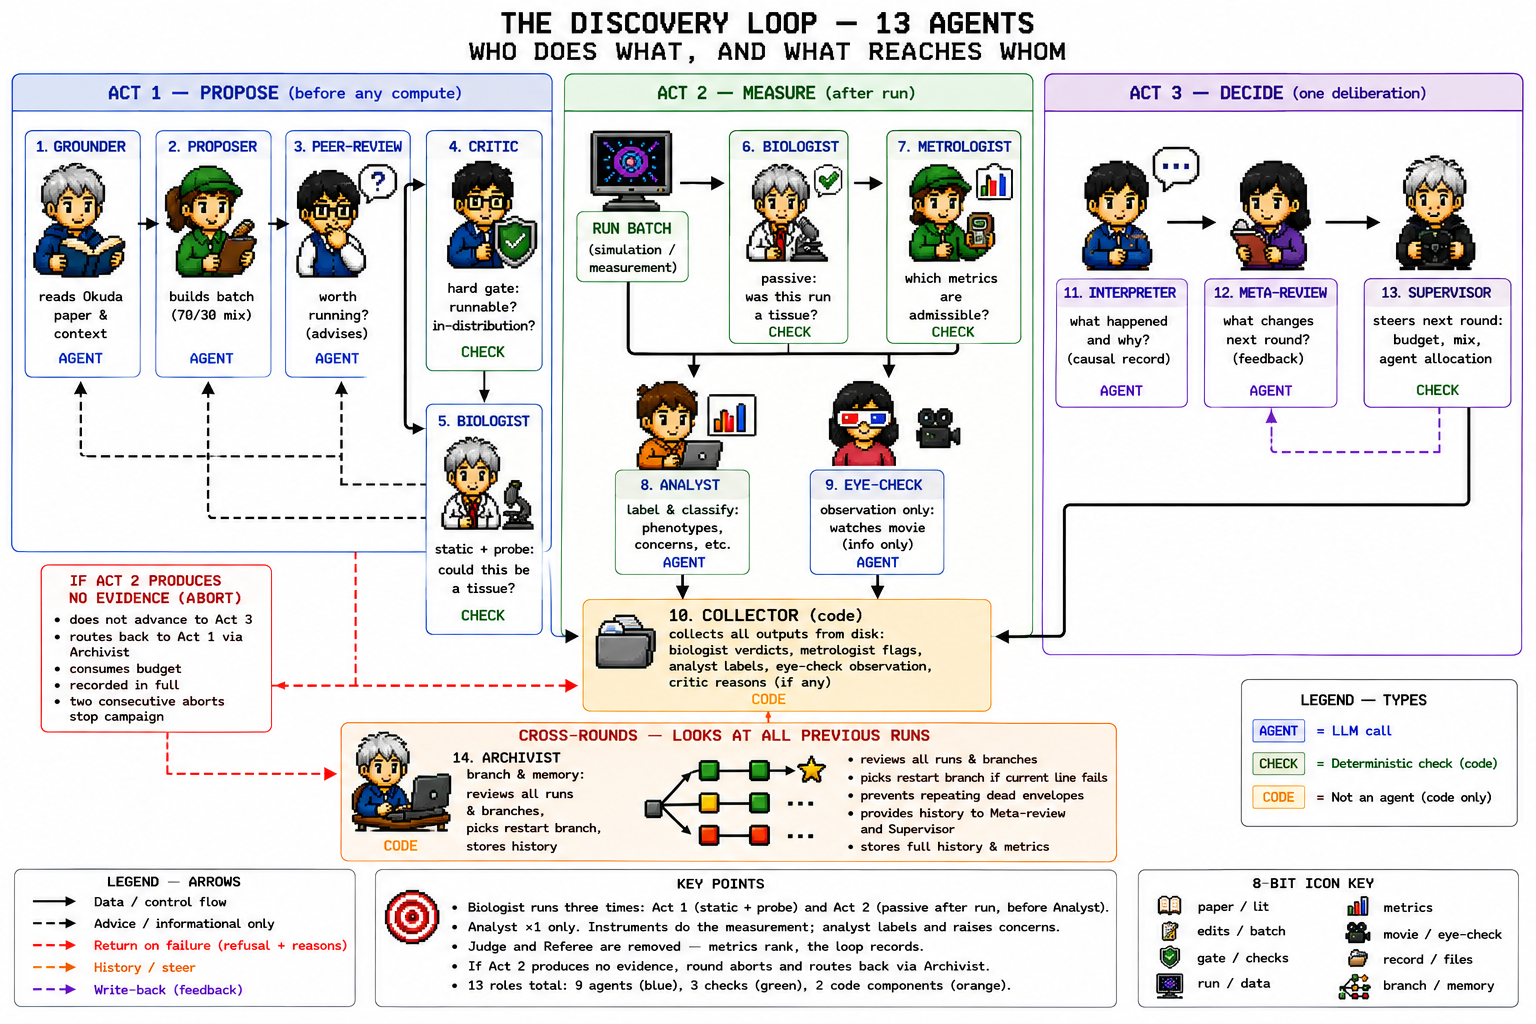
\includegraphics[width=\textwidth]{figures/agentic_loop.png}
\caption*{\small \textbf{The loop after the 1 August rebuild.} Three acts and a cross-round
controller. Blue is an LLM call, green a deterministic check, orange code that is not an agent at
all. \textbf{Thirteen roles in fourteen places} --- the Biologist appears twice, static and probe
before the batch (5) and passive after it but \emph{before} the Reader (6), because a phenotype
named from a specimen whose chemistry was extinct cannot be un-named. The roster is
\code{ROLES.md} and \code{roles.py -{}-check} compares it against the code in both directions.}
\end{figure}

\begin{center}\small
\begin{tabular}{@{}l l p{7.3cm} l@{}}
\toprule
\multicolumn{4}{@{}l}{\textbf{ACT 1 --- Propose.} Before a second of compute is spent.}\\
\midrule
Grounder & agent & what did Okuda actually do? Reads the paper, with its own quotes checked
& \textcolor{warn}{to build}\\
Proposer & agent & which mechanism edits do we test next? Composes the batch under both
mixture rules & runs\\
Peer-review & agent & is this batch \emph{worth} the compute --- falsifiable, not already
settled, a mechanism rather than a restatement of the edit? \textbf{Advises; cannot refuse}
& runs\\
Critic & \textbf{check} & can this be \emph{run}? Type-legal, preconditions met, not already
evaluated, and every scheduled operator actually acted. \textbf{Owns the in-distribution
envelope}: CFL, bounds, stability, admissible ranges & runs\\
Biologist & \textbf{check} & could this be a tissue? Against \code{PREMISES.md}, which it reads
rather than restates. \textbf{Categorical, never prose}: \emph{invalid} on a \textbf{certain}
premise, \emph{ambiguous} on a \textbf{usual} one. \textbf{Static} tier here (the spec alone) and \textbf{probe} (its own
40-frame sim); the \textbf{passive} tier runs in Act 2 & runs\\
\midrule
\multicolumn{4}{@{}l}{\textbf{ACT 2 --- Measure.} The batch runs. The only expensive step.}\\
\midrule
Biologist & \textbf{check} & \emph{was} this run a tissue? The same premises, now against what
the run recorded. \textbf{Runs after the batch and BEFORE the Reader} --- run it after the
analysis and a phenotype has already been named from a specimen whose chemistry was extinct, which
is what happened on \code{r002c\_00}. Nothing can un-name a phenotype & runs\\
Metrologist & \textbf{check} & which metrics are admissible? Certifies instruments against known
answers. \textbf{Owns metric admissibility} --- not the Critic & runs\\
Reader ($\times$1) & agent & what happened in this one run? \textbf{It does not measure --- it
labels.} Every number was computed before it was called, by an instrument the Metrologist
certified, so any number of readers would see the same ones. \emph{Not} Robin's $\times$8: their
Finch writes the analysis code and so produces different \emph{numbers}. \textbf{Settled at one};
what we give up is that nothing records a close call & \textbf{21 s}\\
Eye-check & agent & what does the movie show? \textbf{Observation only --- no veto, no score.}
Its dissent is recorded as a disagreement & runs\\
\midrule
\multicolumn{4}{@{}l}{\textbf{ACT 3 --- Decide.} One deliberation, then act.}\\
\midrule
Collector & \textbf{code} & builds the round record from the files on disk. \textbf{Not an agent:
collection is a \code{for} loop, not a judgement} --- and an agent that collects can forget, in
silence & \textcolor{warn}{to build}\\
Interpreter & agent & what happened this round, and why? \textbf{The causal record}, kept separate
from Meta-review on purpose & runs\\
Meta-review & agent & what should change next round? \textbf{Owns prompt write-back} --- the
feedback appended to the other agents' prompts, which is how Co-Scientist learns without
back-propagation. Writes \code{memory.md} & runs\\
Supervisor & \textbf{check} & what runs next, and how much? \textbf{Owns budget, allocation and
both 70/30 mixtures.} The runtime controller & runs\\
\midrule
\multicolumn{4}{@{}l}{\textbf{CROSS-RUN control} --- outside the acts, over the whole history.}\\
\midrule
\textbf{Archivist} & agent & is the current line worth continuing, or is there a better branch
behind us? \textbf{Reads the whole run history}, not the current batch. Answers
\emph{continue} / \emph{roll back to X} / \emph{stop}. \textbf{Advises the Supervisor; does not
command it} & \textcolor{warn}{to build}\\
\midrule
Cedric & human & looks at the pictures; found every defect so far & outside the loop\\
\bottomrule
\end{tabular}
\end{center}

\vspace{2pt}
\textbf{Dropped: Judge, Referee, Evolution, the duplicate check.} The Judge existed to settle the
Eye-check against the number, and demoting the Eye-check to observation dissolves the dispute; the
Referee ranked by tournament what a certified metric already ranks. \textbf{Both were called zero
times.} \textbf{Evolution} was asked \emph{``what should change next?''} --- and so was the
Meta-review. Two agents answering one question is not a redundant call, it is a roster nobody can
reason about. The surviving split is by \textbf{scope}: Meta-review over \emph{this batch}, the
Archivist over \emph{the whole history}; local refinement of a winner inside the current branch was
the weakest of the three jobs and is the one that went.

\textbf{And the missing role was the historian.} Nothing in the roster ever looked across rounds,
which is why the search could drift down a line with nothing able to say so --- and why the
Proposer could record \emph{``parent 2 is fully PROPOSED''}, counting a family as explored because
it had been \emph{proposed} rather than because anything had been \emph{measured}. Only the history
knows which. The \textbf{Archivist} is also what makes the abort path actionable: a round with no
evidence routes back through it, so the loop can roll back to a better branch instead of
re-proposing inside the envelope the Critic just refused.

\vspace{4pt}
\textbf{Where the hypothesis lives, and who decides whether it held.} This is the discipline the
whole method rests on, and neither paper does it: in Co-Scientist and Robin a hypothesis is
generated, reviewed and ranked, but nothing records what was \emph{believed before the evidence
arrived} --- so a prediction cannot be told apart from a rationalisation written afterwards.

\begin{center}\small
\begin{tabular}{@{}l l p{8.4cm}@{}}
\toprule
\textbf{step} & \textbf{who} & \textbf{what}\\
\midrule
register & \textbf{Proposer} & every slot states a claim, an intent, a named metric and a
prediction \emph{containing a number} --- \code{protr\_peak >= 2.0} --- posed under an id that
cannot be overwritten, before anything is submitted\\
admit the metric & \textbf{Metrologist} & a prediction may only name a metric certified against
known answers. A prediction on an uncertified metric is not a hypothesis, it is a wish\\
catch the uncheckable & \textbf{Peer-review} & the only role whose job is to spot a prediction
that \emph{cannot fail} before the compute is spent\\
\textbf{score} & \textbf{code} (\code{predict.py}) & checked against the measurement
arithmetically. \textbf{No agent decides whether a hypothesis was validated}\\
use & \textbf{Supervisor} & the \textbf{surprise rate} --- how often the prediction was wrong ---
drives the next batch's mixture\\
\bottomrule
\end{tabular}
\end{center}

\textbf{Three outcomes, not two}: \emph{confirmed}, \emph{refuted}, and \textbf{inconclusive} --- a
prediction the code cannot check. Inconclusive is not a soft refutation: it \textbf{drops out of
the surprise denominator entirely}, because a prediction that could not fail teaches nothing and
must not dilute the rate that steers the campaign. The scorer is code for the same reason
everything else here is: a hypothesis scored by an agent is a hypothesis scored by the same kind of
thing that wrote it, and the surprise rate is too central to sit inside a model's discretion.

\vspace{4pt}
\textbf{Which roles serve which track.} The roster is machinery; it exists for two things at once,
and a role that does not know which one it serves will drift.

\begin{center}\small
\begin{tabular}{@{}l p{5.5cm} p{5.5cm}@{}}
\toprule
& \textbf{Track A --- understand the mechanism} & \textbf{Track B --- reproduce Okuda}\\
\midrule
the product & a \textbf{map}: which operator does what & \textbf{the figure}: tube, undulation,
branching\\
measured by & lever-map coverage, and the surprise rate & the scoreboard: how many of the four
morphologies\\
served by & Critic (what is legal), Reader (what happened), Archivist (where to search) &
Grounder (what Okuda did), Biologist (is it a tissue at all)\\
fails by & confirming what we already believe & producing the picture by hand-tuning, which proves
nothing about the method\\
\bottomrule
\end{tabular}
\end{center}

\textbf{The 70/30 in-distribution rule is where the two tracks are allocated, and that is its real
purpose.} \code{in\_paper} slots serve Track~B; \code{excursion} slots serve Track~A. Running only
Okuda's settings teaches us to reproduce his figures rather than to understand the system --- the
objective is a \emph{map, not a target} --- and running only excursions produces understanding of a
model nobody has a reason to believe.

\vspace{4pt}
\textbf{The two mixture rules, each with an owner.} Both are properties of a \emph{batch}, so both
are checked before compute is spent:

\begin{center}\small
\begin{tabular}{@{}l l l@{}}
\toprule
\textbf{rule} & \textbf{composed by} & \textbf{checked by}\\
\midrule
70 confirmatory / 30 adversarial & Proposer & Peer-review\\
70 in-distribution / 30 out-of-distribution & Proposer & \textbf{Critic, deterministically}\\
\bottomrule
\end{tabular}
\end{center}

\emph{In distribution} means the parameter and solver-validity envelope --- CFL, bounds, stability,
numerical sanity --- which is checkable without judgement, and is why it is the Critic's. It does
\emph{not} mean the composition family already explored (the lever map's), nor the regime where the
metrics are certified (the Metrologist's).

\vspace{4pt}
\textbf{A round that produces no evidence is ABORTED, and does not advance to Act 3.} It routes
back to Act 1 carrying the Critic's refusal reasons. It consumes budget and is recorded in full,
but \textbf{does not increment the round counter and enters no coverage denominator} --- counting
it as a normal round is exactly how a log came to tell the Proposer \code{coverage 0\%}, from which
it correctly concluded that its own ledger was broken. \textbf{Two consecutive aborts stop the
campaign and ask}: a second abort means the refusal reasons were not actionable, which is a fact
about us rather than about the search, and without that bound ``route back to Act 1'' is a loop
that burns a week.

\textbf{What the live run actually spent, which is how the roster was judged.} Sixteen calls,
23.5 minutes: \textbf{Proposer 14.8 min} (63\% of all agent time), Peer-review 2.8, Meta-review
2.4, Readers 1.7, and one call each to the Eye-check, Interpreter and Evolution. \textbf{The
Judge and the Referee were never called at all.} That is the measurement the redesign rests on ---
not an argument that they were redundant, but a ledger showing they had nothing to do. Timing was
wired on 1 August; until then nine call sites bypassed the stopwatch and a round once reported
\code{calls: 0} for a round that made about twenty-five. Six real reader calls came in at
\textbf{21 seconds} each against a four-minute allowance and \textbf{7.2 turns} against a cap of
60, so neither the timeout nor the turn cap has ever constrained anything.

%======================================================================
\section{What stands between us and the Okuda figure}\label{sec:okuda}

Most of the gap is mundane and it is about starting conditions. We were running 150 cells where
Okuda starts at 200, 2000 and 4000, and because the mesh buffer is sized as a multiple of the
starting count, beginning at 150 capped every run at 1778 cells --- so his largest case was not
reachable at all. Two of his settings also sat outside the box our search was allowed to use: how
sharply a cell switches on its growth (he uses 10, we allowed up to 8) and how much further the
inhibitor travels than the activator (he uses 10, we allowed 2), and the second is why we could not
produce his handful of well-separated spots. A third number, his pattern length-scale, is not even
the same quantity as ours, so the decision taken with Cedric is to calibrate against what he
\emph{reports seeing} --- the spot count on a ball of a given size --- rather than copy a value
across two differently-scaled models. All of that is four numbers and a buffer, and it is closed in
Phase~2. The one genuine gap is that the coupling only runs one way: chemistry deforms the tissue,
but the tissue's shape never feeds back into the chemistry, because our diffusion averages
neighbours equally instead of weighting by shared wall area and cell volume. A plain tube probably
does not need that arrow --- a tube needs a spot that stays put, and a decal does that perfectly
well. Branching almost certainly does need it, because in Okuda's account a tube forks when the tip
stretches, dilutes its chemical unevenly, and the domain splits. So without it we would not get
branching, and --- worse --- we would not know whether that was a real result or our missing arrow.

%======================================================================
\section{The phases}

Eight stages. \textbf{I stop at the end of each one and wait for you.} That is the partition.

\begin{phasebox}{Phase 0 --- Pre-flight: fix the instruments \hfill \dn\ (28 of 28)}
\textbf{Goal.} Make every measurement trustworthy. Nothing runs unattended until this lands. Not one
of the twenty-eight items is science; each one makes a question \emph{askable}.

\textbf{The last two, closed.} \emph{Comparing a batch at a common frame} --- the per-run evidence
horizon was right and did not make a BATCH comparable. If one run tears at frame 300 and another
holds to 700, comparing their ``final'' states puts a torn mesh beside a healthy one and reports
the difference as biology: both operands valid, the comparison wrong, which is the shape of every
error that has cost this campaign a batch. A batch is now read at one frame, the earliest horizon
in it, and the tool reports what that costs --- how much of each run is discarded, and a warning
when one run's early death is being imposed on everyone. \emph{The explicit vocabulary} ---
\code{elongation}, \code{elongation\_peak}, \code{elongation\_at\_end}, \code{elongation\_unforced}.
Writers emit both names, readers resolve either, the archive is never rewritten: cutting 92
references over in one step leaves a window where a key is written by half the code and read by the
other half, and since an absent metric reads as ``not measured'', the bug would surface as a round
that quietly learns nothing.

\textbf{The repairs worth knowing about}

\footnotesize
\begin{tabular}{@{}l p{11.4cm}@{}}
\toprule
\textbf{what} & \textbf{what was found}\\
\midrule
survival test & It relaxed a fresh sphere and returned 1.014 for every run. Now real:
  \textbf{1.415 $\to$ 1.325, so 94\% of the elongation survived the drivers going off} --- the first
  honest survival number the campaign has produced.\\
the camera & Growth was drawn as \emph{shrinkage}: apparent size fell to 0.52$\times$ on a run that
  grew by half. A second viewpoint justified itself immediately --- in one run \textbf{the tube is
  invisible from the side and obvious from the top}.\\
the tube bar & \textbf{No capsule of any aspect ratio can reach the old bar of 2.0} (ceiling 1.90).
  The criterion was not asking for a tube; it was asking for the spike artefact.\\
damage & The blended damage score was counting \emph{cell division}: sliver correlates with tip
  count at $+0.94$, while genuinely broken cells stayed at \textbf{0 for 300 frames}.\\
the 1778 ceiling & Arithmetic, not physics: $(3552{+}4)/2 = 1778$, and all 32 runs of the overnight
  study stopped there.\\
the missing arrow & The emitter never passed the implementation through --- the ablation would have
  reported ``no effect'' \emph{without ever running the new code}.\\
the curve plot & Drawn every run since the beginning, referenced \textbf{nowhere in the codebase}.\\
timing & The round reported \code{calls: 0} for a round that made about 25.\\
\bottomrule
\end{tabular}
\end{phasebox}

\begin{phasebox}{Phase 1 --- Teach the loop what a tissue is: the premise gate \hfill \dn}
\textbf{Why this became its own phase.} Ten defects were found in one day, every one by Cedric
looking at a picture, and all of the same kind: an operator or an instrument not doing what its name
says. The loop checked that runs finished, that the mesh was valid, that the numbers were finite. It
never once checked that the thing it had simulated was a tissue.

\textbf{Eleven basics, each one something a computer can run and fail}, in three tiers by cost: read
the recipe (instant, refuses a hopeless run before a GPU is touched); read the run (free, goes
loudly into the record); and run a small experiment of its own --- switch everything off and let the
ball sit for forty frames; it must not change size.

\textbf{A broken premise must be declared, not silenced.} Switching off growth to ask what a
protrusion is made of genuinely breaks premise~1, and that is science. So a recipe may waive a
premise \emph{in writing, with a reason}; an undeclared violation is a hard stop. That is the only
thing separating ``we tested an idea'' from ``the settings were wrong''.

\textbf{Every check was proved to fail before being trusted.} The one to look at: run against the
code as it stood that morning, a resting ball collapses \textbf{5.00 $\to$ 0.69} in forty frames.
That single check, which costs about a minute, would have caught the worst defect of the campaign on
day one.
\end{phasebox}

\begin{phasebox}{Phase 2 --- Make Okuda's settings reachable \hfill \dn\ (6 of 6)}
The box used to describe the work without listing it, so the count had no visible
denominator. All six, with what each one turned out to be:

\footnotesize
\begin{tabular}{@{}r@{.\ }p{5.0cm} l p{6.3cm}@{}}
\toprule
& \textbf{item} & \textbf{state} & \textbf{what it turned out to be}\\
\midrule
0 & The ball could not get big enough & \dn &
  \emph{Not on the list.} A spring held the shell at the size it was first built at while the cells
  inside grew sixteen-fold, so the sheet folded through itself. The spring's target now follows
  what the cells are asking for: the same run grows smoothly to 5\,240 cells and stays clean.\\
1 & Widen the out-of-range settings & \dn &
  Done, and the new bounds are \emph{derived} rather than chosen: growth sharpness to 49.5
  (Okuda needs 10), inhibitor spread to 12.5 (he needs 10), reaction speed unbounded.\\
2 & Replace the mislabelled length-scale & \dn &
  The quantity we called a pattern size is a solver rate. Resolved in Phase 4 by measuring the
  pattern instead of setting it.\\
3 & The shape-to-chemistry feedback & \dn &
  One contract, four implementations --- curvature, tension, apical area, pressure --- because
  \emph{which} feature the chemistry listens to is the hypothesis, not a dial. Force and size were
  refused with reasons.\\
4 & A fixture asserting his published constants & \dn &
  His Table 1 is now written down in the Grounder, quoted, with the sentence each value comes
  from --- the Hill coefficient, the two diffusivities, the cell cycle, and the two regime
  \emph{inequalities} that actually define his setting. Asserting a run against it is Phase 3,
  because it needs the Grounder wired.\\
5 & His cell counts, with the buffer sized for the \emph{destination} & \dn &
  \textbf{The item that voided the weekend batch}, and it is measured rather than argued ---
  see below.\\
\bottomrule
\end{tabular}

\normalsize
\textbf{Item 5, tested rather than argued.} A closed cell sheet is trivalent, so Euler fixes the
vertex count at twice the cell count: a reservoir of 3552 vertices caps the tissue at
$(3552{+}4)/2 = 1778$ cells exactly, whatever the biology wants. The reservoir is now computed from
the count a run is \emph{aiming at}. The same recipe, run twice, with nothing changed but the seed
count and the reservoir:

\begin{center}\small
\begin{tabular}{@{}l r r r l@{}}
\toprule
& \textbf{seeds} & \textbf{vertex buffer} & \textbf{cells at end} & \textbf{verdict}\\
\midrule
before & 150 & 3\,552  & \textbf{1778} & saturated --- not evidence\\
after  & 200 & 10\,404 & \textbf{4151} & clean --- valid evidence\\
\bottomrule
\end{tabular}
\end{center}

The old configuration stops dead on the rail; the new one grows past Okuda's largest case.
Elongation is 1.061 against 1.073, so the physics is unchanged --- the run simply gets to happen.
Sizing the buffer from the seed instead of the destination is what produced 1778 twice in one week.

\textbf{One error the check caught on me.} My first version sized the reservoir from the seed
count, which gave the 200-cell case a ceiling of 264. Okuda is explicit that his largest tissues
were ``picked up on the growth process'' --- a destination, not a start --- so the two are now
recorded as separate numbers.

\textbf{Certification caught two of my own errors} on item 3 --- a curvature normalisation that only
looked right because the test held cell count fixed, and a test of mine that demanded the wrong
answer.

\textbf{The phase closes on a green self-test, which it did not have an hour ago.} The composition
space checks itself in 61 ways, and eight were failing --- silently, since yesterday. Seven were the
growth-ceiling fix and the chemistry-clock fix diverging from the archived recipes: the space is
right and the archive is wrong, so both are now \emph{declared} deliberate rather than back-fitted
into the archive, because rewriting a reference to make a test pass is how it stops being one. The
eighth was real --- no reference recipe used the new shape-to-chemistry operator, so the recipe
named for Okuda's route was missing the half that makes it his. It carries it now. And the
chemistry clock, previously exempt and unchecked, gained a test of its own: both terms must scale
by exactly $1/\mathrm{dt}$ \emph{and} their ratio must be unchanged, since that ratio is what sets
the Turing wavelength. \textbf{61 of 61.}
\end{phasebox}
\begin{phasebox}{Phase 3 --- Switch on the agents that never run \hfill \dn\ (3 of 3)}
\textbf{Ablation is now compulsory} --- \emph{done}, and it is the part that matters. A claim that
one thing \emph{causes} another needs two experiments and we were enforcing neither: adding a
mechanism and seeing the shape appear shows it is \emph{sufficient}; taking it away and seeing the
shape die shows it is \emph{necessary}. Either alone is an opinion.

Every claim must now declare its kind, and the checker throws out a batch that asks for more than it
tests --- before any simulation starts. Sufficient earns ``is sufficient for''; necessary earns ``is
required for''; both earn ``causes''; neither earns ``is associated with''. \textbf{The word can no
longer outrun the experiment.}

\textbf{Still to do --- and one of the three is now the priority.}

\textbf{(a) Wire the Grounder} --- \emph{done}. It is the only agent that reads the paper and it
had no call site anywhere; every entry point was exercised only by its own smoke test. Batch
construction now asks it, and it answers with Okuda's own numbers: 2,000 cells,
carrying the sentence they came from. It arrives as
a \emph{parameter}, so composition identity is unchanged --- setting the starting size is a retune,
not a new mechanism, and the search cannot mistake one for the other.

Two rules keep it from becoming a straitjacket. The Grounder \emph{advises}: the faithful share of
a batch inherits his numbers, the exploratory share is free to leave them --- a search that may
only ever stand where the paper stands cannot discover that the paper is not the only place to
stand. What is \emph{not} optional is the reservoir, and that lives in the translator where it
applies to both shares alike.

\textbf{And it was wrong the first time, in the most dangerous way available.} My first version
started tubulation at 200 cells, quoting the paper. The sentence was real; the mapping was not.
``About 200 cells'' belongs to two \emph{control} experiments Okuda runs first --- one on arrested
tissue that cannot grow at all, one with growth decoupled from the morphogen. His three morphology
figures are a single coupling experiment at \textbf{2,000} cells, and only $\chi$ and $\gamma$
separate them. Cedric caught it. A quotation is not a citation: the quote made a tenfold error look
verified, which is worse than having offered no quote at all. There is now no case to infer --- a
slot either declares which of Okuda's experiments it is, or it gets the coupling one.

Still open here: asserting a run against his published constants. The values are written down;
nothing yet checks a run against them.

\textbf{(b) Evolution and the Referee} --- \emph{done}. \code{rank\_btl} had been written and
self-tested since the loop was built and had never ranked a real batch; the round sorted on
whichever scalar the instrument gate happened to admit. A tournament decides now. Verified on a
synthetic batch: a vetoed run holding the highest score drops from first to last. Evolution runs
too, refining the winner rather than the loop only ever \emph{picking} from what the enumerator
offered.

\textbf{(c) The per-run calls run together} --- \emph{done, and measured}. Runs are read
concurrently across a batch, and the machinery for reading one run $N$ ways in parallel remains,
because no reader's prompt depends on another's answer.

\textbf{$N$ is now 1, and the reason it was three did not survive being examined.} Three readings
were justified by Robin's eight, and Robin's Finch \emph{writes the analysis code} --- it chooses
the flow-cytometry gating and the RNA-seq filters, so its trajectories produce genuinely different
\emph{numbers}. Ours writes none: by the time a Reader is called, \code{diag.json}, the curve shapes
and the strip were computed by instruments the Metrologist certified, and every reader would see
identical numbers. What varies is the \emph{label} --- phenotype, forced-or-grown, the concern
raised --- so $N$ readings would measure \textbf{phenotype ambiguity}, a real quantity but a much
smaller prize than the one the argument was imported for. What we give up at one, stated plainly:
nothing records when a label was a close call. The count is a single number and raising it is one
line.

The eye-check still runs \emph{after}, because it is handed the reading and is not independent ---
parallelising a dependency is not an optimisation, it is a different experiment.
\end{phasebox}

\begin{phasebox}{Phase 4 --- Measurements that can tell his regimes apart \hfill \dn}
\textbf{The classifier} --- \emph{done}. Sphere, undulation, tube, branched, plus \textbf{invalid}
(the surface passes through itself, so no shape reading means anything) and \textbf{unclear},
returned deliberately near a boundary. A classifier that always answers can never be wrong, and one
that can never be wrong teaches nothing. ``Invalid'' beats every morphology --- this campaign has
already once reported a crumpled shell as a result. It records the \emph{path} a run takes, not just
where it ends.

\textbf{It has since become the arbiter} (Phase 4d), replacing the labels a person wrote from the
movies --- a stronger ground truth, not merely a cheaper one, because it is certified against
shapes whose answer is known \emph{by construction}. Until 1 August nothing called it: built,
certified, never asked. Every run now carries its shape and its path beside its numbers.

\textbf{The calibration, and the surprise.} The plan was to tune until we saw Okuda's handful of
spots on a 2000-cell ball, then freeze. Counting spots over time --- for the first time --- showed
something else:

\begin{center}\small
\begin{tabular}{@{}lrrrrrr@{}}
\toprule
step        & 0 & 50 & 100 & \textbf{200} & 400 & 3000\\
spots       & 104 & 62 & 19 & \textbf{7} & 1 & 1\\
coverage    & 0.06 & 0.14 & 0.37 & 0.49 & 0.52 & 0.53\\
\bottomrule
\end{tabular}
\end{center}

\textbf{The pattern never settles.} It keeps merging until the ball is one connected blotch covering
half the surface. So ``about five spots'' was a passing moment around step 200, not a property of
the settings --- and calibrating to it by choosing when to stop would have produced a number that
looked right and meant nothing. The chemistry this campaign has always used makes \emph{mazes}, not
spots. Nobody noticed because nothing counted spots, and the movie's colour scale was rescaled every
frame, so a merging pattern and a stable one looked identical in both the numbers and the pictures.

The calibration became a search for where stable spots actually live, tested by counting at two
well-separated times. Twenty settings; the winner gives three spots that stay three spots across
three independent runs, and is frozen as the default.
\end{phasebox}

\begin{phasebox}{Phase 4b --- Can the chemistry be simulated at all? \hfill \dn}
\textbf{Why this became a phase, mid-flight.} The pre-launch stopped on a run whose chemistry
turned to infinities within a hundred frames. Chasing that found the rule which exists to prevent
exactly this, and it had been \textbf{fifty times too generous} for as long as the campaign has
existed.

\textbf{What the rule is for.} Two chemicals sit on the cell sheet: one that builds up and makes
more of itself, and one that spreads further and suppresses it. The simulation moves them a little
at a time. If a single step moves too much at once, the arithmetic runs away and every number
becomes infinite --- and everything measured afterwards describes the solver rather than the
tissue. There is a standard condition for how much movement per step is too much. It depends on
two settings: a \emph{spreading multiplier} that scales both chemicals together, and how far the
suppressing chemical travels.

\textbf{What went wrong.} The condition was written down as a \emph{comment}, worked out once, for
the settings of the day. Then the defaults changed, and Phase 2 deliberately widened the range so
Okuda's own values would be reachable at all --- and the arithmetic in the comment quietly stopped
describing the code. A comment cannot be re-derived. It can only be re-read, and nobody had cause
to re-read it. On top of that it counted one factor twice, reporting a fiftieth of the true figure.

\textbf{What it cost.} \code{okuda\_route} --- the recipe named for the target --- was four times
past the safe limit and passed every check in the system. Its chemistry died within a hundred
frames, and the Biologist refused every run that used it. That refusal is the only reason this was
found: no metric would have shown it, because there were no numbers left to look at.

\textbf{Then it was tested against the engine, and the corrected rule was still wrong.} Twenty
runs on the cluster, three hundred frames each, across the predicted boundary. An argument about
where a limit lies is worth nothing until the boundary it predicts is the one the engine has:

\begin{center}\small
\begin{tabular}{@{}r r l l@{}}
\toprule
\textbf{spreading} & \textbf{suppressor} & \textbf{what actually happened} & \\
\textbf{multiplier} & \textbf{range} & & \\
\midrule
0.01 & 10   & healthy pattern & \textbf{Okuda's own value works}\\
1.3  & 0.16--0.42 & healthy pattern & the working band\\
3    & 0.16 & healthy pattern & \\
\midrule
0.05 & 10   & \textcolor{bad}{infinities} & predicted safe\\
1.3  & 0.5  & \textcolor{bad}{infinities} & \\
4    & 0.16 & \textcolor{warn}{fine, but dead} & no pattern at all\\
6    & 0.16 & \textcolor{warn}{fine, but dead} & \\
\bottomrule
\end{tabular}
\end{center}

\textbf{One number cannot express the limit, because there are two ways to fail and it knows
about one.} Running away is the one it forbids. The other is that the chemicals spread so readily
that the pattern smears out and dies --- the simulation stays perfectly well behaved and measures
nothing. \textbf{Well behaved is not the same as alive}, and no stability condition sees the
difference.

\textbf{So the rule is now two conditions, and both were measured rather than derived.} The step
size must be under the limit, \emph{and} the spreading multiplier must stay under three. The second
has no formula behind it --- it came from watching fourteen settings run. It exists because the
multiplier scales both chemicals at once, so turning it up flattens the self-reinforcing chemical's
own peak as fast as it spreads the suppressor, and past about three the peak cannot outrun its own
spreading.

Okuda's own setting for how far the suppressor travels \emph{is} reachable --- it sits in the first
row of the table above, at a low spreading multiplier.

\textbf{The limit sits below the first failure we saw.} The measurements do not fall either side of
a clean line --- two settings above it ran fine, one below it did not --- so the rule refuses two
combinations known to be good.

That is the safe direction, and it is worth being explicit about which one is which. A
\emph{permissive} rule admits a setting that then fails: the run happens, produces numbers, and
those numbers are about the solver. That is how thirty-two runs and then twenty-seven more became
findings before anyone noticed. A \emph{strict} rule refuses a setting that would have been fine,
and costs one proposal. The old rule was permissive by a factor of fifty; this one errs strict
until the term that explains the odd case is found.

Checked against all eight settings that were run: every bad one refused, no bad one admitted.

\textbf{Still to do}
\begin{itemize}[itemsep=1pt]
\item \textbf{Find the missing term.} Two settings cannot order the failures on their own, and the
rule stays conservative until something explains the case that breaks the pattern.
\item \textbf{The reaction has no limit at all}, on purpose --- a candidate was proposed, measured
and refuted --- so a recipe can pass this check and still die through the reaction instead.
\item \textbf{Longer runs may move the boundary.} These were judged at three hundred frames. A run
that survives three hundred and dies at nine hundred is still a run the gate let through.
\item \textbf{One trusted recipe sits on the wrong side.} \code{round\_44\_base} ran healthily by
hand --- nine hundred frames, three thousand cells, a strong pattern --- and is four times past the
limit when rebuilt as a composition, because the clock repair speeds its chemistry up fiftyfold.
Both are true, and they are not the same experiment: the archived run had a fiftieth of the
reaction time the repair gives, which is the very defect the repair was written for. Keeping it as
a reference keeps a pre-repair run among the trusted ones. The self-test sits at 54 of 56 on
exactly this, and the decision is Cedric's.
\end{itemize}

\textbf{Whose job this is.} The \textbf{Critic}. It is deterministic, it runs before any compute,
and it already refuses a recipe that is illegal, unrunnable or already tried --- ``cannot be
simulated'' is the same kind of statement. Not the Metrologist, who certifies that an
\emph{instrument} measures what it claims, and not the Biologist, who asks whether the
\emph{specimen} is a tissue. This one asks whether the arithmetic can be carried out at all, which
is a property of the proposal, and the proposal is what the Critic reads.
\end{phasebox}

\begin{phasebox}{Phase 4c --- Multi-spot initialisation, and replication \hfill \dn}
\textbf{Why.} Cedric: \emph{``did you forget to run multiple tubes from now on, not a single
one''}. He is right, and the note already said so --- one protrusion per run is a single sample,
and you cannot tell ``this mechanism makes tubes'' from ``this run made a tube''. Several spots
give within-run replication for free, and it is what Okuda shows. Every control I built during
the pre-launch used one spot or none.

\textbf{Measured}, six runs at the stable point, 300 frames:

\begin{center}\small
\begin{tabular}{@{}r r r l@{}}
\toprule
\textbf{seed fraction} & \textbf{act\_max} & \textbf{activated fraction} & \\
\midrule
0.02 & 0.423 & 0.40 & \\
0.06 & 0.501 & 0.37 & three seeds, \textbf{identical to 3 d.p.}\\
0.15 & 0.598 & 0.12 & \\
0.30 & \textcolor{bad}{0.000} & 0.10 & the pattern is extinguished (P4)\\
\bottomrule
\end{tabular}
\end{center}

\textbf{Two findings, one of them a problem.} Seeding more widely does not give more pattern --- it
gives \emph{less}, and past 0.15 it gives none at all: a seed covering a third of the shell leaves
no room for the inhibitor to separate domains, so the whole field decays together. The useful band
is narrow and sits below 0.15.

\textbf{And the three seeds were bit-identical} --- 0.501, 0.501, 0.501. \code{general.seed} was
written into every spec and read by \emph{nothing}: both stochastic operators take a \code{seed}
(the mesh jitter, and which cells are nucleated) and the translator passed neither. ``Three
independent runs'' were one run repeated, so every spread this campaign has quoted across seeds
described the floating-point reproducibility of a single trajectory.

\textbf{Fixed, and the fix follows the working specs rather than my first idea.} I offset the two
operators' seeds, reasoning that jitter and nucleation are independent draws. True, and beside the
point: \code{archive\_rounded.py}, \code{archive\_vh\_rd\_coral.py} and \code{run\_tyssue\_fig5.py}
all pass \emph{one shared} SEED to both, and a composition that reproduces an archived run has to
draw the numbers that run drew. Departing from the convention would have made every reproduction
check compare two different experiments. A spec that declares a seed no operator consumes is now
refused outright.

\textbf{Replication, measured for the first time} --- three seeds, 300 frames, same composition:

\begin{center}\small
\begin{tabular}{@{}l l l l@{}}
\toprule
& \textbf{act\_max} & \textbf{activated fraction} & \textbf{elongation}\\
\midrule
before & 0.501,\ 0.501,\ 0.501 & 0.374 $\times$3 & 1.006 $\times$3\\
after  & 0.501,\ 0.447,\ 0.483 & 0.407,\ 0.379,\ 0.374 & 1.006,\ 1.006,\ 1.005\\
\midrule
       & sd \textbf{0.022} & sd \textbf{0.015} & sd 0.0005\\
\bottomrule
\end{tabular}
\end{center}

That last row is what a difference between two compositions now has to beat to mean anything. It
did not exist yesterday, and every claim made without it was comparing single samples.
\end{phasebox}

\begin{phasebox}{Phase 4d --- The picture stops voting \hfill \dn}
\textbf{Cedric's call, and it removes what had been blocking the loop.} The metric bank was
certified by making numbers reproduce labels written from the \emph{movies}, and a vision model's
reading of a movie could drop a run out of the ranking entirely. Movies stay --- the model still
watches every run, and a disagreement between the picture and the numbers is the only signal in
the loop that comes from looking at shape rather than at numbers. What they no longer do is
\emph{decide}.

\textbf{Two reasons beyond the call.} The veto was circular: the eye-check was handed the
reader's label --- derived from the same caption it then read --- so it could catch a
summariser drifting from a caption and could not catch numbers disagreeing with reality, which is
what it was credited with. And the camera was broken for the whole period the veto was trusted:
one fixed viewpoint, and a zoom re-fitted to the tissue every frame, so growth was drawn as
shrinkage and a tube could sit behind the body. A gate reading a broken instrument is worse than
no gate.

\textbf{What arbitrates instead.} The morphology classifier, which answers \emph{which of Okuda's
shapes is this} from geometry and is certified against shapes whose answer is known by
construction --- a built sphere is a sphere, nine built bumps are an undulation, an extruded tube
is a tube, a forked one is branched, and a self-intersecting shell is refused a label at all.
Nobody's opinion enters. Alongside it, the Biologist: a run that fails a premise is not a tissue
and cannot calibrate an instrument.

\textbf{What this costs, honestly.} The eye-check vetoing the top two runs of round 2 was reported
as the system's best moment. It becomes a \emph{recorded disagreement} instead --- which is the
truthful version, since the camera it was reading was showing growth as shrinkage at the time.
The disagreement is still written down, and it is still worth reading.
\end{phasebox}

\begin{phasebox}{Phase 5 --- The first live run: the agents do not talk to each other \hfill \prog}
\textbf{It ran, and that is the point.} Two rounds, eight simulations, 23 agent calls, 29
minutes of agent time. \textbf{One usable run. Map coverage 0\%.} Nothing was learned about the
biology --- and the reason turns out to be worth more than the biology would have been.

\textbf{What the machine got right, unprompted.} The Critic refused every bad run and named the
reason. The straggler killer cut two runs at 46 minutes against an 11-minute batch median. The
Supervisor diagnosed its own sterility --- \emph{``surprise 0.00: the batch is confirming what we
already believe, near-zero information. Push adversarial''} --- and a round with nothing
admissible said so instead of scoring what it had.

Every one of those is a correct judgement. \textbf{Not one of them reached another agent.}

\subsection*{The diagnosis: written by somebody, read by nobody}

The Proposer's own reasoning for round 4, verbatim, is the whole case:

\begin{quote}\small
``Header shows round 3, 0 runs, coverage 0\% \ldots another \textbf{counter-reset artifact}; real
record = memory.md.''\\[2pt]
``Those two batches proposed ALL FOUR valid single-op edits on parent 2, so parent 2 is
\textbf{fully PROPOSED} and \ldots cannot be built on further.''
\end{quote}

It was handed a summary built only from the lever map, and the lever map is filled \emph{after}
the Critic --- so a refused run contributes nothing to it. Eight simulations had died of diverged
chemistry and saturated buffers, and the Proposer was told ``0 runs, coverage 0\%''.

It then drew the only sane conclusion available from an insane input: that the \emph{ledger} was
broken, and its own prose memory was the real record. And it counted a family as explored because
it had \textbf{proposed} the edits, not because it had \textbf{measured} anything --- so it moved
on to a fresh parent believing the previous one was mapped, when nothing had been learned there
at all.

\textbf{An audit of every hand-off found the same shape seven more times:}

\begin{center}\small
\begin{tabular}{@{}l l l@{}}
\toprule
\textbf{who produces it} & \textbf{what} & \textbf{who receives it}\\
\midrule
Critic        & every refusal, with its reason      & \textcolor{bad}{nobody}\\
Supervisor    & ``push adversarial'', the mix steer  & \textcolor{bad}{the terminal, only}\\
Interpreter   & \code{causal\_descriptions.md}       & \textcolor{bad}{nobody}\\
Evolution     & \code{evolution.jsonl}, its refinement & \textcolor{bad}{nobody}\\
Grounder      & Okuda's starting conditions          & \textcolor{bad}{the config, not the Proposer}\\
scoreboard    & \code{scoreboard.md}, the headline product & \textcolor{bad}{never written by a round}\\
lever map     & \code{lever\_map.md}                 & \textcolor{bad}{nobody}\\
\bottomrule
\end{tabular}
\end{center}

And the instruction the Proposer works from names three admitted metrics, of which the
\code{ta\_*} family is \textbf{absent from half the runs on disk} --- so it writes predictions
that cannot be scored, which resolve \emph{inconclusive} and drop out of the surprise rate
entirely. The loop is measuring its own information rate with a ruler that discards the
measurements.

\subsection*{The reason, stated once}

The campaign was built as a set of roles, each with a job, each doing it. What was never built is
the \emph{wiring}. Every agent writes; almost nothing reads. The result is not a loop but a fan:
work flows outward from the Proposer and never returns, so the system cannot be corrected by its
own findings. \textbf{A loop that is told only about its successes cannot avoid repeating its
failures} --- and this one had no successes to be told about.

That also explains the day's other defects, which looked unrelated and are not: a refusal printed
among hundreds of lines, an evidence horizon silently absent, a buffer flag raised after the
compute was spent, a state file grown past reading, a black movie. Each is a correct output with
no recipient.

\textbf{Drawing it is what made the shape obvious.} Every agent's output was plotted against
whoever read it, and the picture was a fan rather than a loop: work flowed outward from the
Proposer and almost nothing came back. Fourteen roles, and the only thing they shared was the
direction of travel. That picture is what turned the repair from ``wire these hand-offs'' into
``why are there so many hand-offs to wire'' --- which is \S\ref{sec:agents}, and Phase~6.

\subsection*{Fixed}

\textbf{Refusals are now evidence.} The Proposer receives what ran, what was refused and the
reason code, with the distinction stated plainly: an empty map beside a non-zero attempt count is
not a reset counter --- it means the compositions proposed so far \emph{cannot be simulated}, a
parent is explored when its edits produced evidence and never when they were merely proposed, and
the refusal codes say what to change.

\textbf{The black movie.} The colour scale is computed once for the whole run --- correctly, since
a per-frame rescale makes a decaying pattern and a stable one look identical --- but over samples
including non-finite values, and one of those makes both bounds non-finite. \textbf{Frame 0 was
perfectly good and was drawn black because frame 800 diverged.} The artefact reported ``nothing
happened'' for a run whose first half was fine. Now: finite values only, cells that left the model
drawn grey rather than white, and the count said out loud.

\textbf{The Biologist now speaks to somebody.} It had been running on every run since it was
written, and its verdict went to a terminal and to a field of \code{diag.json} that no prompt has
ever mentioned. On round 2 it broke five premises on the very run whose movie came out black ---
\emph{the activator had decayed to NaN, the chemistry was extinct} --- and a Reader read that
run's numbers and named a phenotype. Two hand-offs now exist: the per-run verdict goes to the
\textbf{Reader} that is about to read it, in the document's own words and with a field it must
fill in saying whether the specimen was sound; and the round-level tally goes to the
\textbf{Meta-review}, whose whole job is the recurring pattern. Across round 2 that tally reads
\emph{``P4 broken in 2 of 3 runs''} --- an edit family that cannot hold chemistry, which is a thing
to stop proposing rather than a thing to keep measuring.

\textbf{And the premises are read from \code{PREMISES.md}}, not retyped beside it. Two documents
saying the same thing in different words will disagree, and the one that drifts is always the prose
--- it is the one nothing executes. The titles, grades and stated checks now come from the
document, and the drift is reported in both directions. It found two immediately: premise~10
(neighbour exchange is rare) is written down and \textbf{nothing checks it}, and \code{P12} is
checked on every run and \textbf{appears nowhere in the document}.

\textbf{The two written records have a shape}, checked rather than suggested: an append-only log
with per-round fields, beside a state document of seven named sections. \code{memory.md} had
reached 1904 words across six appended blocks in a file whose purpose is to hold state.

\subsection*{What the diagnosis led to}

Wiring the hand-offs one at a time was the wrong repair, and stopping to ask \emph{why there were
so many to wire} was the right one. The answer is in \S\ref{sec:agents}: sixteen roles copied from
a system that runs no experiments. \textbf{The roster was rebuilt --- thirteen roles, three acts,
Judge and Referee dropped, the Collector made code} --- and the design is written down in
\code{ROLES.md} so that this decision cannot evaporate the way the Biologist's verdicts did.

\subsection*{Still to wire}
\begin{itemize}[itemsep=1pt]
\item \textbf{The Collector} --- the round record, built from disk. Everything below lands on it.
\item The Supervisor's steer into the Proposer's prompt, not the terminal.
\item The Grounder into the Proposer's prompt, rather than into the config.
\item The Critic's deterministic 70/30 in-distribution gate.
\item The abort path: no evidence $\rightarrow$ back to Act 1, two in a row $\rightarrow$ stop.
\item The Interpreter's descriptions and Evolution's refinement into the next round's evidence.
\item The admitted-metric list rebuilt from what runs actually record.
\item The reservoir target from the growth a composition asks for --- three of eight runs
outgrew an estimate the gate then correctly refused, one step too late.
\item The scoreboard written by the round that changes it.
\end{itemize}
\end{phasebox}

\begin{phasebox}{Phase 6 --- The rebuilt loop, and its first launch \hfill \prog}
\textbf{Goal.} Launch the three-act loop of \S\ref{sec:agents} and let it run. Phase~5 diagnosed
why the old one could not learn; this is the one that is allowed to try.

\subsection*{What was built}
\begin{itemize}[itemsep=1pt]
\item \textbf{The Collector} (\code{collector.py}) --- code, not an agent. It assembles the round
record from the files on disk and \textbf{writes \code{analysis.md}}, which the Proposer used to
write about itself. Every field is measured or quoted; it composes no prose. It also reports its
own \emph{holes} --- \code{[collector] HOLE: r003c\_01: the Biologist never ran on it} --- because
the point of building a record from disk is that a missing input becomes visible rather than
silent.
\item \textbf{The Archivist} (\code{archivist.py}) --- the role the roster never had. It reads the
whole history, answers \emph{continue} / \emph{roll back} / \emph{stop}, and runs on every abort.
All the arithmetic is done in code and handed over as a table; only the choice is put to a model.
\item \textbf{The abort path.} A round with no admissible evidence no longer advances to Act~3:
it is recorded in full, \textbf{does not increment the round counter}, routes back through the
Archivist, and \textbf{two in a row stop the campaign} with exit code~3, which the driver treats
as terminal rather than retrying.
\item \textbf{The three return paths} the Proposer never had: the Supervisor's steer, the Critic's
refusals \emph{with their reasons}, and the Grounder's starting conditions from the paper --- each
a prompt section that disappears when empty rather than saying ``none'' in ten lines.
\item \textbf{Judge, Referee and Evolution deleted} from the code, not merely unwired.
\textbf{Reader $\times$1}, renamed for what it does. The \textbf{Biologist} now returns a
categorical verdict --- \emph{invalid} on a \textbf{certain} premise, \emph{ambiguous} on a
\textbf{usual} one --- decided by the grade in \code{PREMISES.md} rather than by judgement.
\item \textbf{\code{memory.md} moved to the Meta-review}, on an enforced template. Neither record
is the Proposer's any more.
\end{itemize}

\subsection*{What the cold start found, and what it cost to misread it}

The loop now begins by asking the Archivist where to start from what is on disk. The first thing
it did was read \code{mechanics.npz}, which nothing had ever read: \textbf{across all 63 finished
runs, \code{n\_protruding} never once exceeded zero and \code{protr\_peak} never exceeded 1.13.}
The summary had been reporting ``best sound run 1.11'', which reads like a result and is a sphere
with noise on it. \textbf{This project has never produced a protrusion}, and the number saying so
sat in every run's mechanics file, unread, for the whole campaign.

\textbf{Then it gave up --- and that was the expensive mistake, and it was ours.} It ranked every
candidate on \code{protr\_peak} and \code{n\_protruding}, found zeros, and fell back to
\code{okuda\_route}. Those are \textbf{Track~B} measures: they say whether we made Okuda's picture.
\textbf{Track~A asks a different question}, about the landscape of operators, and a composition
that runs, patterns and holds a sound specimen is a point on that map whether or not anything
protruded. Judging a Track~A starting point by a Track~B criterion, and then treating a Track~B
zero as the end of the road, is how the fallback recipe became the starting point three separate
times. \textbf{Measured on the corrected ranking: 46 of 63 runs serve Track~A.} The campaign had
46 usable starting points and was reporting that it had none. \emph{Track~A does not run out} ---
so \code{stop} is now stated as a Track~B verdict only.

\subsection*{Three defects the batches themselves surfaced}

\textbf{Two operators where one was meant.} \code{impl\_structural} marked an operator whose
implementation is a real mechanism choice \emph{and} was read as permission to hold two of them,
so the menu offered both \code{+shape\_energy\_3d:default} and \code{=shape\_energy\_3d:default}.
The Proposer took the add and wrote the claim for the swap; the spec came out with two whole
mechanics solvers driving the same vertices. Closed in the generator and, separately, in the
Critic --- a guard that lives only in the generator is a guard against one way of being wrong.

\textbf{A stale proposal, silently adopted.} \code{proposal.json} was six seconds older than the
process that read it. The harness's read-before-write rule blocked the overwrite, the agent read
the file and reported \emph{``already holds a complete, valid Round-1 proposal \ldots\ no rewrite
is needed''}, then verified it against every rule and ran it. The guard against clobbering had
become a mechanism for inheriting stale work. The file is now deleted before the call, so there is
nothing to inherit.

\textbf{And the one that killed the batch.} The activator went $0.01 \to 1.41\times10^{6} \to$
NaN \textbf{while spatially uniform} --- spread $3.4\times10^{-5}$ against a mean of $1.4\times
10^{6}$. A diffusion breach makes a checkerboard; a uniform blow-up is an ODE exploding. The CFL
was 0.208 against a limit of 0.45 and was never the problem. There was a bound on diffusion and
\textbf{none on the reaction}. One probe at \code{dt=1.0} disproved the clock theory that looked
obvious, and the discriminator is single-variable across three runs: \code{gierer\_meinhardt}
explodes, \code{gray\_scott} patterns --- and \code{okuda\_route}, the recipe named for the target,
carries the former.

\subsection*{The Diagnostician, and why it is a role}

Cedric's objection, and it is correct: \emph{``we cannot launch, crash, and do this every time''}.
Every one of those diagnoses was done by hand. The Biologist can say a specimen is invalid and the
Metrologist that an instrument is uncertified; \textbf{neither can say why the apparatus failed},
so a human did the forensics after every crash --- which is not autonomy, it is manual work moved
later. The \textbf{Diagnostician} computes when each series went non-finite, whether the divergence
was \emph{spatial or uniform}, which runs share the signature, and \textbf{what differs between a
failing run and the nearest passing one} --- the step that isolated \code{chi 65 vs 1.3} with every
other parameter equal. It returns \code{cause}, \code{evidence}, \code{guard\_to\_add} and
\code{stop|continue}, runs \emph{before} the Interpreter, and can halt the campaign.

\subsection*{The launch: reconnaissance first}

The first round \textbf{sets no hypotheses}. The Proposer picks six specs already on disk from the
Archivist's ranked table and they are re-run \emph{verbatim} --- no edits, no predictions, intent
\code{control}, resolving \code{inconclusive} so they leave the surprise denominator. There is
nothing to be surprised by in a replay, and a prediction attached to one would be a prediction
about our own past arithmetic. Every number we held was taken with at least one instrument since
proved wrong; the product is a frontier of compositions we have \emph{seen work}, measured with
instruments we are entitled to believe.

\subsection*{It ran. Three rounds, then the same six specs again}

\begin{center}\small
\begin{tabular}{@{}l l r r l@{}}
\toprule
& \textbf{when} & \textbf{evidence} & \textbf{refused} & \textbf{specimens}\\
\midrule
round 1 & 22:34 & 3 & 3 & all valid\\
round 2 & 22:55 & 2 & 4 & all valid\\
round 3 & 23:16 & 3 & 3 & all valid\\
\bottomrule
\end{tabular}
\end{center}

Three \emph{distinct} rounds --- \code{r001n}, \code{r002n}, \code{r003n} all on disk together,
the counter advancing --- at $\sim$21 minutes each, of which $\sim$5.5 is agent time. Every act
ran every round: Collector, Interpreter correctly declining a replay, Meta-review, Archivist. The
refusals are \code{P2\_BUFFER\_SATURATED} on the stale-reservoir specs: the Critic working, not a
failure.

\textbf{The moment worth the day} was round~2, the first time the Archivist had history to reason
over: \emph{``continue --- sole branch is sound 3/3, best 1.01 sphere --- \textbf{a valid Track~A
operator point}; no better branch''}. It read a sphere at \code{protr\_peak 1.01} as a legitimate
point on the operator map rather than a failure. Ranking exactly that number \emph{as} a failure is
what made the cold start give up three times over.

\textbf{And then Cedric asked why it kept running the same spec.} It did: four rounds, the same six
or seven runs with a swap or two. Three things made that inevitable and none of them is a bug ---
the Archivist's ranked table is \textbf{static}, since re-measuring a run does not change its
pattern quality; nothing told the Proposer what it had \emph{already replayed}; and recon poses no
predictions, so the surprise rate stays null and the map cannot grow. The Archivist had said so
itself in round~2, in one phrase: \emph{``sole branch''}.

\textbf{Reconnaissance is a one-shot and I had it rolling to forty.} One round establishes the
frontier; every round after it must be \code{composition}, which is the mode that proposes an edit,
predicts a number and can be \emph{wrong} about it. \code{campaign\_loop.py} is now phased ---
\code{-{}-recon-rounds} defaults to 1 --- and the two shell drivers written beside it are deleted.
Bash cost two errors in an evening, one of them editing a script \emph{while bash was executing
it}, which re-reads by byte offset and corrupted the running instance.

\subsection*{What is running now, and what it is a test of}

Twenty rounds: one reconnaissance to rebuild the frontier, then composition. \textbf{The first
composition round is the first time anything in this project poses a falsifiable prediction and
can be wrong about it} --- and the first use of the parents that reconnaissance produced, now that
\code{composition.json} ships beside every spec.

\textbf{What to watch}: whether the surprise rate is ever non-null (a campaign that only confirms
has bought coverage and no knowledge), the Collector's holes, and whether any run reports a
protruding cell --- which would be the first in the project's history, across 63 prior runs and
these.
\end{phasebox}

\begin{phasebox}{Phase 7 --- The demonstration \hfill \todo}
\textbf{Goal.} Run the designed grid --- six to eight simulations --- that produces the figure:
tube, undulation and branching, at Okuda's settings.

\textbf{What you get.} \emph{The figure.}
\end{phasebox}

\begin{phasebox}{Phase 8 --- The method claim \hfill \todo}
\textbf{Goal.} Write up what the loop found by itself versus what we told it, with the record of
predictions and retractions as the evidence.

\textbf{What you get.} The argument that Track A works, resting on Track B.
\end{phasebox}

%======================================================================
\section{The 31 July lesson, in three lines}

Ten defects in one day, every one found by Cedric looking at a picture and none by the loop --- a
ball that shrank to nothing, a movie where every cell turned green at once, a coral that began
uniformly red. They were all the same kind: the loop could tell whether a \emph{simulation}
succeeded and had never been able to tell whether the \emph{specimen} was a tissue. Phase~1 is the
answer to exactly that, and the only way to find out whether it is enough is to run a batch and see
whether the gate catches anything before Cedric does.

%======================================================================
\section{What I need from you}

Nothing blocking. Two things worth knowing:

\begin{enumerate}[leftmargin=1.4em]
\item \textbf{The buffer gate is the one decision worth taking now.} Phase 5 has already been
spent once on runs that could not have produced evidence. A pre-launch refusal costs nothing and
would have saved the batch.
\item \textbf{Tell me if this note is the right shape.} Too long, too short, wrong order --- it is
cheap to change, and it is the thing that lets you steer.
\end{enumerate}

%======================================================================
\section*{Appendix --- words I could not avoid}

Only these four. Everything else above is ordinary English.

\begin{itemize}
\item \textbf{Cell sheet (or mesh)} --- the model of the tissue: a hollow ball of polygonal cells
sharing walls, like a football.
\item \textbf{Operator} --- one mechanism as a reusable building block: ``cells divide'',
``chemical spreads'', ``surface pulls tight''. A model is a combination of these.
\item \textbf{The loop} --- the automated cycle: propose a change, predict the outcome, run,
measure, record whether the prediction held.
\item \textbf{Phase} --- one of the eight stages above. Our agreed stopping points.
\end{itemize}

\subsection*{The four measurements, renamed}

Agreed 31 July. The old names misled in three separate ways and are being retired: \code{protr}
reads as a length but is a \emph{ratio}; \code{final} became ambiguous the moment we introduced
the evidence horizon; and \code{Q} said nothing at all. The rename happens as one mechanical pass
once the current work lands, with old records aliased on read --- the archive is never rewritten.

\begin{center}\small
\begin{tabular}{@{}l l p{7.9cm}@{}}
\toprule
\textbf{was} & \textbf{is} & \textbf{means}\\
\midrule
\code{protr} & \code{elongation}
& the 95th-percentile cell radius divided by the median. \textbf{1.0 is a sphere.} A ratio, not a
length --- reading 1.62 as an amount of protrusion is the mistake the old name invited.\\
\code{protr\_peak} & \code{elongation\_peak}
& the most elongated it ever got, over \emph{valid} frames only.\\
\code{protr\_final} & \code{elongation\_at\_end}
& at the last \emph{valid} frame --- not simply the last frame.\\
\code{Q} & \code{elongation\_unforced}
& what remains after growth and pushing are switched off and the tissue relaxes.
\textbf{This is the forced-versus-grown test}, and it is the whole reason the campaign exists: we
can already make a tube by pushing; the question is whether the tissue will hold one by itself.\\
\bottomrule
\end{tabular}
\end{center}

\vspace{6pt}
\hrule
\vspace{6pt}
{\small\color{grey}
My working log is \texttt{SESSION\_LOG.md}; the findings register is \texttt{findings.py} and the
premises are \texttt{PREMISES.md}. You should not need any of them.}

\end{document}
